% Этот шаблон документа разработан в 2014 году
% Данилом Фёдоровых (danil@fedorovykh.ru) 
% для использования в курсе 
% <<Документы и презентации в \LaTeX>>, записанном НИУ ВШЭ
% для Coursera.org: http://coursera.org/course/latex .
% Исходная версия шаблона --- 
% https://www.writelatex.com/coursera/latex/2

\documentclass[a4paper,12pt]{article}

%%% Работа с русским языком
\usepackage{cmap}					% поиск в PDF
\usepackage{mathtext} 				% русские буквы в формулах
\usepackage[T2A]{fontenc}			% кодировка
\usepackage[utf8]{inputenc}			% кодировка исходного текста
\usepackage[english,russian]{babel}	% локализация и переносы

%%% Дополнительная работа с математикой
\usepackage{amsfonts,amssymb,amsthm,mathtools} % AMS
\usepackage{amsmath}
\usepackage{icomma} % "Умная" запятая: $0,2$ --- число, $0, 2$ --- перечисление

%% Номера формул
%\mathtoolsset{showonlyrefs=true} % Показывать номера только у тех формул, на которые есть \eqref{} в тексте.

%% Шрифты
\usepackage{euscript}	 % Шрифт Евклид
\usepackage{mathrsfs} % Красивый матшрифт

%% Свои команды
\DeclareMathOperator{\sgn}{\mathop{sgn}}

%% Перенос знаков в формулах (по Львовскому)
\newcommand*{\hm}[1]{#1\nobreak\discretionary{}
{\hbox{$\mathsurround=0pt #1$}}{}}

%%% Работа с картинками
\usepackage{graphicx}  % Для вставки рисунков
\graphicspath{{images/}{images2/}}  % папки с картинками
\setlength\fboxsep{3pt} % Отступ рамки \fbox{} от рисунка
\setlength\fboxrule{1pt} % Толщина линий рамки \fbox{}
\usepackage{wrapfig} % Обтекание рисунков и таблиц текстом

%%% Работа с таблицами
\usepackage{array,tabularx,tabulary,booktabs} % Дополнительная работа с таблицами
\usepackage{longtable}  % Длинные таблицы
\usepackage{multirow} % Слияние строк в таблице
\usepackage{titlesec}
\usepackage[left=1.27cm,right=1.27cm,top=2cm,bottom=2cm]{geometry}


%%% Заголовок
\author{Кожарин Алексей}
\title{Копипаста с работ Эйлера}
\date{\today}

\begin{document}
	\maketitle
	\stepcounter{section}
	\titleformat{\paragraph}[runin]
	{\normalfont\bfseries}
	{}
	{0pt}
	{\S\,}
	\paragraph{2} 
	Пусть фиг. \ref{fig21} представляет собой положения Солнца $S$, Земли $T$ и Луны $L$, и пусть $\Theta$ есть центр тяжести Земли и Луны. Делаем следующие обозначения:
	
	\begin{table}[h]
		\label{definitions}
		\caption{Обозначения}
		\begin{center}
			\begin{tabular}{rlcc}
				Масса & Солнца & \dots & $S$ \\
				>> & Земли & \dots & $T$ \\
				>> & Луны & \dots & $L$
			\end{tabular}
		\end{center}
	\end{table}

	Расстояние:
	\[
	S \Theta = \rho\,;~ ST = \rho_1\,;~ SL = \rho_2\,;~ TL = r
	\]
	тогда будет:
	\begin{equation}
	\label{eq1}
		\begin{aligned}
			T \Theta = r_1 = \frac{L}{T+L} r \\
			L \Theta = r_2 = \frac{T}{T+L} r
		\end{aligned}
	\end{equation}
	Составим теперь выражения ускорений, которые эти тела сообщат друг другу.
	\begin{figure}[!h]
		\centering
		\label{fig21}
		\caption{}
		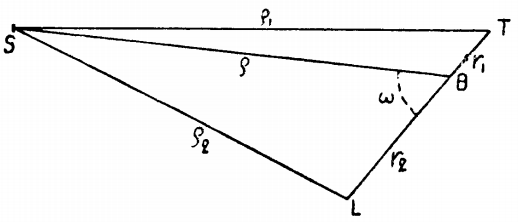
\includegraphics[width=0.45\linewidth]{fig21}
	\end{figure}

	%\newpage	% Если что, верните его!
	Солнце $S$ сообщает ускорения:
	\begin{table}[!h]
		\centering
		\begin{tabular}{rcccc}
			Земле: & $f \cdot \cfrac{S}{\rho_1^2}$ & по & направлению & $TS$ \\[5mm]
			Луне: & $f \cdot \cfrac{S}{\rho_2^2}$ & >> & >>  & $LS$
		\end{tabular}
	\end{table}

	\noindent  чего точка $\Theta$ имеет ускорения:
	\newpage
	\begin{table}[!h]
		\centering
		\begin{tabular}{rcccc}
			$\cfrac{T}{T+L} \cdot f \cdot \cfrac{S}{\rho_1^2}$ & по & направлению, & параллельному & $TS$ \\[5mm]
			$\cfrac{T}{T+L} \cdot f \cdot \cfrac{S}{\rho_2^2}$ & >> & >> & >> & $LS$
		\end{tabular}
	\end{table}

	Ускорения Солнца, происходящее от притяжения Земли и Луны, соответственно, суть:
	\begin{table}[!h]
		\centering
		\begin{tabular}{cccc}
			$f \cdot \cfrac{T}{\rho_1^2}$ & по & направлению & $ST$ \\[5mm]
			$f \cdot \cfrac{T}{\rho_2^2}$ & >> & >> & $SL$ \\			
		\end{tabular}
	\end{table}
	
	\noindent поэтому ускорения точки $\Theta$ относительно точки $S$ будет:
	\begin{table}[!h]
		\centering
		\begin{tabular}{ccccc}
			$w_1 = f \cdot \cfrac{(S + T + L)}{T + L} \cdot \cfrac{T}{\rho_1^2}$ & по & направлению & параллельно & $TS$ \\[5mm]
			$w_2 = f \cdot \cfrac{S+T+L}{T+L} \cdot \cfrac{L}{\rho_2^2}$ & >> & >>		   & >>			 & $LS$
		\end{tabular}
	\end{table}
	
	\noindent Разлагая эти ускорения, соответственно, по направлениям $\Theta S$ и $\Theta L$, получим, как легко видеть из подобия показанных на фиг. \ref{fig22} и \ref{fig23} треугольников:
	\begin{table}[!h]
		\centering
		\begin{tabular}{cccc}
			$w_1 ' = w_1 \cdot \cfrac{\rho}{\rho_1}$ & по & направлению & $\Theta$ S \\[5mm]
			$w_1 '' = w_1 \cdot \cfrac{r_1}{\rho_1}$ & >> & >> & $\Theta L$ \\[5mm]
			$w_2 ' = w_2 \cdot \cfrac{\rho}{\rho_2}$ & >> & >> & $\Theta S$ \\[5mm]
			$w_2 '' = w_2 \cdot \cfrac{r_2}{\rho_2}$ & >> & >> & $L \Theta$
		\end{tabular}
	\end{table}
	\begin{figure}[!h]
		\centering
		\label{fig22}
		\caption{}
		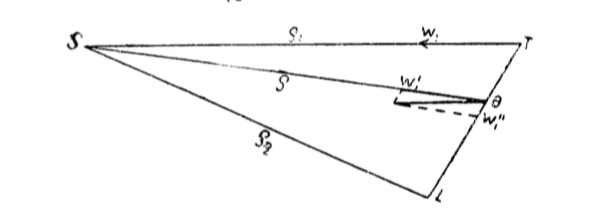
\includegraphics[width=0.6\linewidth]{fig22}
	\end{figure}

	получим для ускорений точки $\Theta$ слагающие:
	\newpage
	\begin{table}[!h]
		\centering
		\begin{tabular}{ccc}
			$W_1 = w_1' + w_2' = f \cdot \cfrac{S + T + L}{T + L} \cdot \left[ T \cdot \cfrac{\rho}{\rho_1^3} + L \cdot \cfrac{\rho}{\rho_2^3} \right]$ & по & $\Theta S$ \\[5mm]
			$W_2 = w_1'' - w_2'' = f \cdot \cfrac{S + T + L}{T + L} \cdot \left[ T \cdot \cfrac{r_1}{\rho_1^3} - L \cdot \cfrac{r_2}{\rho_2^3} \right]$ & по & $\Theta L$ \\
		\end{tabular}
	\end{table}
	\begin{wrapfigure}{l}{0.4\textwidth}
		\centering
		\label{fig23}
		\caption{}
		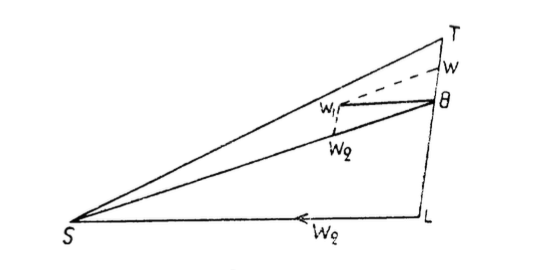
\includegraphics[width=\linewidth]{fig23}
	\end{wrapfigure}

	%\newpage
	Заменив $r_1$ и $r_2$ их выражениями (\ref{eq1}), имеем:
	
	\begin{align*}
	& W_1 = f \cdot \cfrac{S + T + L}{T + L} \cdot \rho \cdot \left[ \dfrac{T}{\rho_1^3} + \dfrac{L}{\rho_2^3}\right] \text{по направлению } \Theta S \\
	& W_2 = f \cdot \cfrac{S + T + L}{\left(T + L\right)^2} \cdot T \cdot L \cdot r \left[ \dfrac{1}{\rho_1^3} - \dfrac{1}{\rho_2^3}\right] \text{по направлению } \Theta L
	\end{align*}
	
	Но

	\begin{align*}
		& \rho_1^2 = \rho^2 + 2 \rho \cdot \cfrac{L}{T+L} \cdot r \cos \omega + \left(\dfrac{L}{T+L} \cdot r\right)^2 \\
		& \rho_2^2 = \rho^2 - 2 \rho \cdot \cfrac{L}{T+L} \cdot r \cos \omega + \left(\dfrac{L}{T+L} \cdot r\right)^2
	\end{align*}
	следовательно:
	
	\begin{align*}
	\dfrac{1}{\rho_1^3} = \dfrac{1}{\rho_3} \left[1 + 3\,\dfrac{L}{T+L} \cos \omega + \left( \dfrac{L}{T+L} r\right)^2 \left(-\frac{3}{2} + \cfrac{15}{2} \cos^2 \omega\right) + \dots\right] \\
	\dfrac{1}{\rho_2^3} = \dfrac{1}{\rho_3} \left[1 + 3\,\dfrac{T}{T+L} \cos \omega + \left( \dfrac{T}{T+L} r\right)^2 \left(-\frac{3}{2} + \cfrac{15}{2} \cos^2 \omega\right) + \dots\right]
	\end{align*}
	Подставляя эти выражения, имеем:
	
	\begin{align*}
	& W_1 = f \cdot \dfrac{S + T + L}{\rho^2} \left[1 + \dfrac{T \cdot L}{\left(T + L\right)^2} \cdot \dfrac{r^2}{\rho^2} \left( - \frac{3}{2} + \frac{15}{2} \cos^2 \omega \right) + \dots\right] \\
	& W_2 = f \cdot \dfrac{S + T + L}{\rho^2} \left[-3 \cdot \dfrac{T \cdot L}{\left(T + L\right)^2} \cdot \dfrac{r^2}{\rho^2} \cos \omega + \dots\right]
	\end{align*}
	Но отношения
	
	\begin{alignat*}{3}
	\frac{L}{T+L} \approx \frac{1}{80}; \quad &
	\frac{r}{\rho} \approx \frac{1}{400}; \quad &
	\left(\frac{r}{\rho}\right)^2 = \frac{1}{160000}
	\end{alignat*}
	поэтому будет
	
	\[
		\frac{T \cdot L}{\left(T + L\right)^2} \cdot \frac{r^2}{\rho^2} \approx \frac{1}{12800000}
	\]
	и члены, содержащие этот множитель, могут быть отброшены, так что будет:
	
	\begin{align*}
	& W_1 = f \cdot \frac{S+T+L}{\rho^2} \text{ по направлению } \Theta S \\
	& W_2 = 0 \text{ по направлению } \Theta L
	\end{align*}
	
	Отсюда следует, что точка $\Theta$ движется вокруг Солнца по эллиптической орбите по законам Кеплера.
	
	Рассмотрим теперь ускорение Луны по отношению к Земле, для чего к ускорениям, сообщаемым Луне Солнцем и Землею, надо присовокупить ускорение, равное и противоположное ускорению Земли, происходящему от действия Солнца и Луны. Поступив подобно предыдущему, получим:
	
	\[
	f \cdot \frac{T + L}{r^2} + f \cdot S\left[\frac{r_2}{\rho_2^3} + \frac{r_1}{\rho_1^3}\right] \text{ по направлению } L\Theta \\
	\]
	\[
	f \cdot S \cdot \rho \left[\frac{1}{\rho_2^3} - \frac{1}{\rho_1^3}\right] \text{ параллельно } \Theta S
	\]
	положим:
	\[
		T + L = \mu; \quad S = M
	\]
	
	\listoftables
	\listoffigures	% merde
\end{document}